\subsubsection{Понятие эффекта и системы эффектов}

Центральным определением в данной работе, является, разумеется, \term{эффект}. Однако несмотря на то, что это определение, судя по всему, было введено еще на заре развития программирования (так, ранние работы по аксиоматизации программирования уже ссылаются на этот термин без отдельного его введения \cite{Hoare69, Schwartz67}), общепринятой формулировки за все это время не появилось. 

В классических источниках, под эффектом чаще всего понимают <<некоторое видимое изменение в окружении>> \cite{Luc88}, или даже еще более конкретно <<изменение в памяти программы>> \cite{Vak09}. Некоторые исследователи и вовсе ограничивают это определение до <<чтения или записи в изменяемое состояние программы>> \cite{Green99}. Это можно резюмировать следующим образом:

\begin{definition}
\label{def-effect-1}
    \term{Эффектом} называется некоторое изменение, производимое подпрограммой в состоянии вычислителя (кроме возвращения подпрограммой значения).
\end{definition}

Другие же авторы употребляют более широкую трактовку <<эффекта>> \cite{Nielson99}: 

\begin{definition}
\label{def-effect-2}
    \term{Эффектом} является описание действий, происходящих в ходе выполнения подпрограммы.
\end{definition}

Разумеется, формулировка \ref{def-effect-2} является слишком широкой -- вплоть до того, что под нее подходит непосредственно исходный код тела функции. С другой же стороны, формулировка \ref{def-effect-1} является нежелательно узкой в контексте данной работы. Поясним это на примере. 

Рассмотрим следующую функцию, которая является тривиальной оберткой над проверкой переменной на принадлежность строковому типу:

\begin{minted}{kotlin}
fun isString(x: Any?): Boolean {
    return (x is String)
}
\end{minted}

И рассмотрим следующий участок кода:

\begin{minted}{kotlin}
if (isString(t)) {
    ...
}
\end{minted}

Мы хотели бы сказать, что в истинной ветке условного оператора мы наблюдаем тот эффект, что <<\code{isString} вернула значение \code{true}>>. Однако это действие не подходит под определение эффекта \ref{def-effect-1}. Мы могли бы отказаться от специального случая для возвращаемых значений в этой формулировке, но в дальнейшем мы встретим некоторые утверждения, которые мы тоже хотели бы называть эффектами, но которые не описывают вообще никакого изменения в состоянии вычислителя.

Поэтому нам понадобится определение, чуть более слабое, чем определение \ref{def-effect-1}, но при этом не являющееся чересчур расплывчатым, как \ref{def-effect-2}. Мы сформулируем его следующим образом:

\begin{definition}
    \label{def-effect}
    \term{Эффект} -- это некоторая информация об окружении, получаемая при выполнении подпрограммы.
\end{definition}

Т.к. это определение рассматривает только окружение, то сразу отпадают все слишком широкие его интерпретации. В частности, все, что подпрограмма делает со своими локальными переменными, не подходит под это определение -- что очень удобно, т.к. изменения в локальных переменных нас никоим образом не интересуют.

С другой стороны, это определение включает в себя определение \ref{def-effect-1}, т.к. <<изменение в состоянии>>, несомненно, является <<информацией об окружении>>.

Наконец, как мы увидим чуть позже, под это определение подходят и довольно нестандартные действия, которые нам будет удобно считать эффектами во имя общности подхода.


\bigskip

Естественным продолжением определения эффекта является определение \term{системы эффектов}. Само по себе название уже достаточно интуитивно, особенно если провести параллель <<эффект также относится к системе эффектов, как тип относится к системе типов>>. Тем не менее, мы дадим здесь формальное определение, т.к. это понятие также является центральным в данной работе и будет многократно использоваться в дальнейшем:

\begin{definition}
    \term{Система эффектов} -- это множество правил, по которым подпрограммам и их конкретным вызовам приписываются эффекты, и по которым осуществляется взаимодействие эффектов.
\end{definition}




\subsubsection{Анализ потока данных}

Кроме того, нам в дальнейшем нам понадобятся основные концепции data-flow анализа.

Начнем с понятия графа потока управления (англ. \eng{control-flow graph, CFG}) Каждая инструкция в нем представлена одной вершиной, и если между вершинами $u$ и $v$ есть ребро, то это означает что после инструкции $u$ управление может быть передано 
в инструкцию $v$. 

Рассмотрим простой пример кода:

\begin{minted}{kotlin}
    if (x == 0) {
        println("True branch")
    } else {
        println("False branch")
    }
    println("If-end")    
\end{minted}

Ему соответствует граф потока управления, как на рисунке \ref{control-flow-example}

\begin{figure}
    \centering
    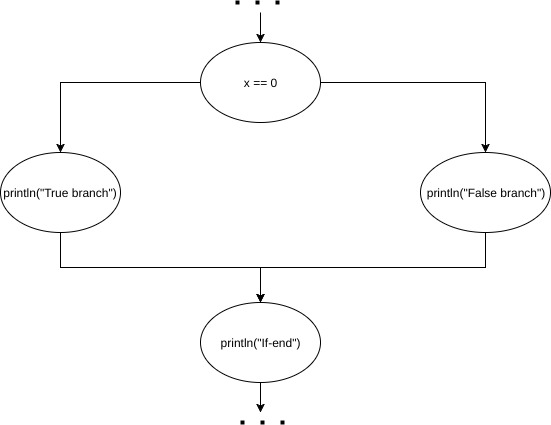
\includegraphics[scale=0.5]{img/control-flow-example}
    \caption{Пример графа потока управления}
    \label{control-flow-example}
\end{figure}


Так, после инструкции, вычисляющей условие в \code{if}, поток управления раздвоился, отражая тот факт, что мы не можем знать при статическом анализе (без дополнительных предположений), какая из веток выполнится. После ветки вновь сливаются в один поток, как и следовало ожидать.

Разумеется, граф потока управления не обязан быть ацикличным -- конструкции \code{for}, \code{while}, \code{goto} (безусловных переход) могут вносить в него обратные ребра.

Важно заметить, что любому возможному пути исполнения в программе обязательно соответствует некоторый путь в CFG, но обратное не верно. Например, путь может проходить через истинную ветку выражения \linebreak \code{if (x == 0) } и через истинную ветку выражения \code{if (x != 0)}, хотя между первым и вторым оператором могло и не быть никаких изменений переменной \code{x}, и иногда это даже можно доказать статически.
Тем не менее, это не нарушает консервативности анализа, поскольку при анализе будет обязательно рассмотрен любой реально возможный путь исполнения. 

Конструкция графов потока управления сама по себе позволяет обнаружить совсем простые ошибки, вроде недостижимого кода из-за неправильного использования безусловных переходов. Однако она становится особо мощной и полезной, если использовать ее вместе с концепцией анализа потока данных.

\begin{definition}
	Анализ потока данных (англ. \eng{data-flow analysis})  -- это метод статического анализа, который основывается на извлечении информации из характеристик и свойств потока данных вдоль различных путей исполнения в программе.
\end{definition}

Основная идея основывается на наблюдении, что в любой момент времени при выполнении программы существует некоторое глобальное состояние, которое состоит из множества всех переменных, их значений, а также другой информации, зависящей от конкретного типа анализа (например, счетчик количества вызовов для функций, статус инициализации переменной, и т.д.). Тогда для каждой точки программы можно ввести понятие \term{значения потока данных} (от англ. \eng{data-flow value}), которое является абстракцией всех возможных глобальных состояний, которые можно наблюдать в данной точке. Для краткости, в дальнейшем мы будем писать DFV вместо <<значение потока данных>>.

В силу того, что потенциально количество возможных путей исполнения в программе может быть бесконечно \cite{dragon-book}, на практике делается два упрощения: во-первых, конкретное DFV не хранит историю, как управление могло придти к этой точке программы, а во-вторых, в зависимости от конкретного анализа, откидывается некоторая излишняя информация. Так, например, при анализе инициализации переменных, нам не важно, какие значения может иметь переменная, и на каких путях исполнения они могли быть получены. Достаточно знать, правда ли, что на любом пути исполнения, достигающем данную точку, данная переменная была инициализирована, или нет. Таким образом, для каждой переменной достаточно просто хранить бинарный флаг, что значительно упрощает реализацию на практике.

Далее, каждой инструкции $s$ соответствует \term{входное состояние} -- глобальное состояние непосредственно перед выполнением инструкции, которое мы будем обозначать $in[s]$, и \term{выходное состояние} -- соответственно, глобальное состояние непосредственно после выполнения инструкции (его мы будем обозначать $out[s]$). Обратим внимание, что выходное состояние для одной инструкции является входным для следующей, с котором она соединена ребром в CFG. Каждому входному (выходному) состояние соответствует некоторое DFV, и в силу предыдущего факта, это отображение является сюръекцией, но не биекцией.

Кроме того, каждая инструкция задает некоторое преобразование, называемое \term{функцией перехода} (англ. \eng{transfer function}), которое по входному состоянию выдает выходное. Конкретный вид преобразования определяется анализом и самой инструкций. 

Таким образом, мы получаем набор уравнений на переменные $in[x]$, $out[x]$ для всех $x \in I$, где $I$ -- множество инструкций в программе. Хотелось бы получить некоторое решение этих уравнений, т.е. множество значений для входных-выходных состояний, удовлетворяющее этим уравнениям. Мы не будем вдаваться в подробности того, как это делается, т.к. это иррелевантно к данной работе, подробней про методы решения систем уравнений на поток данных можно прочитать в канонических источниках: \cite{dragon-book, muchnick}. В дальнейшем нам будет достаточно концепции графа потока управления, входных-выходных состояний и функций перехода.
